\section{Implementierung}
In diesem Kapitel wollen wir auf die Implementierung unseres Prototypen eingehen.


\subsection{Vorstellung des Ablaufs}
Zunächst beschreiben wir dazu den grundsätzlichen Ablauf des Prozesses anhand einer Skizze:
\begin{figure}[H]
\centering
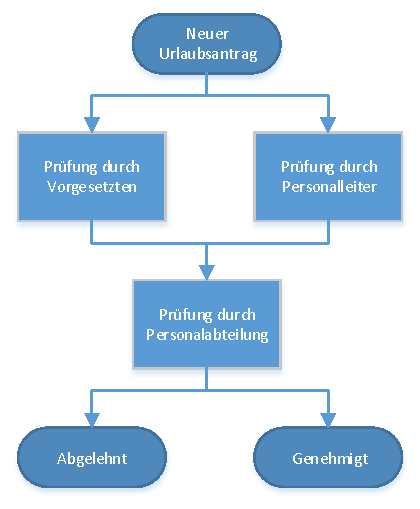
\includegraphics[width=0.5\linewidth]{Bilder/Workflow}
\caption{Skizze des Prozessablaufs}
\label{fig:Workflow}
\end{figure}

Hat ein Mitarbeiter einen Urlaubsantrag ausgefüllt startet ein neuer Urlaubsgenehmigungsprozess. Der Antrag muss an verschiedenen Stellen geprüft werden. In unserem Beispielunternehmen muss der Urlaubsantrag durch den Vorgesetzten und ggf. dem Leiter der Personalabteilung genehmigt werden. Da die Reihenfolge hierbei keine Rolle spielt, können die beiden Schritte parallel ausgeführt werden. Abschließend prüft die Personalabteilung, ob der Mitarbeiter noch über genügend freie Urlaubstage verfügt und genehmigt bzw. verweigert den Antrag.	
	
	
\subsection{Systemübersicht}
Abbildung \ref{fig:Komponenten} stellt eine Übersicht unseres Systems dar. Um einen neuen Urlaubsgenehmigungsprozess starten zu können, müssen zunächst die erforderlichen Daten wie Name, Anzahl der Tage und Urlaubstyp vom Mitarbeiter eingegeben werden. Diese Daten werden im Urlaubsantragsobjekt Application, was über die Schnittstelle UserInterface angelegt wird, gespeichert.

\begin{figure}[H]
\centering
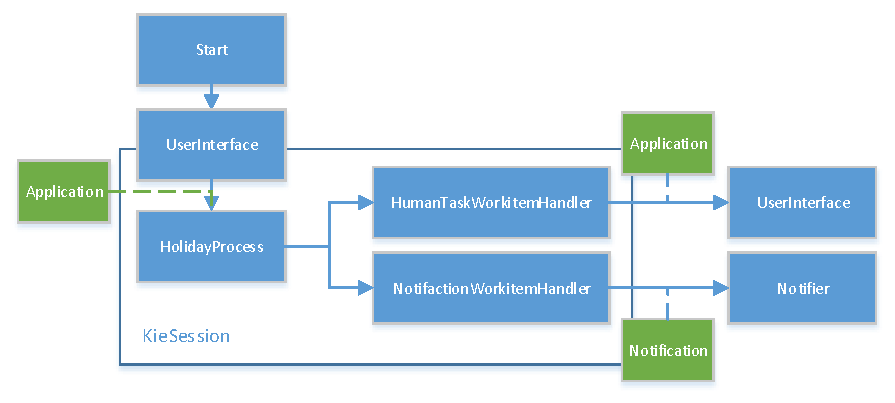
\includegraphics[width=1.0\linewidth]{Bilder/Komponenten}
\caption{Eine Übersicht der beteiligten Komponenten}
\label{fig:Komponenten}
\end{figure}

Nach Eingabe der Daten, wird eine neue KieSession erzeugt und ein neuer HolidayProcess gestartet. Dieser benötigt zur Abarbeitung der Workflow-Schritte insgesamt zwei WorkItemHandler. Der HumanTaskWorkItemHandler realisiert die Interaktion mit dem Endanwender und benötigt dazu die Schnittstelle UserInterface. Dabei werden die eingegebenen Daten ebenfalls in dem Datenobjekt Application gespeichert. Der NotificationWorkItemHandler ist für die Benachrichtigung der Mitarbeiter zuständig und verwendet dazu die Schnittstelle Notifier. Daten die für das Benachrichtigen von Mitarbeitern relevant sind werden in dem Datenobjekt Notification gespeichert.

Das verwendete Datenmodell und die benötigten Schnittstellen werden in den folgenden Abschnitten nun näher beschrieben.

\subsubsection{Datenmodell}
Wie Abbildung \ref{fig:Datenmodell} zeigt, besteht unser Datenmodell insgesamt aus zwei Klassen:

\begin{figure}[H]
\centering
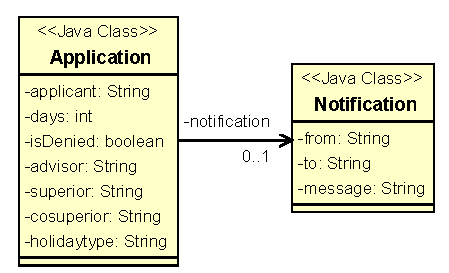
\includegraphics[width=0.5\linewidth]{Bilder/Datenmodell}
\caption{Datenmodell unserer Anwendung}
\label{fig:Datenmodell}
\end{figure}

In der Klasse Application werden alle Daten gespeichert, die für den Urlaubsantrag relevant sind. Neben dem Antragssteller (applicant) werden die Anzahl der Werktage (days) und der Typ des Urlaubs (holidaytype) gespeichert. Zudem ist der Vorgesetzte (superior), der Stellvertreter (cosuperior) und der zuständige Sachbearbeiter (advisor) hinterlegt. Außerdem speichern wir den Antragsstatus (isDenied) und eine dazugehörige Benachrichtigung (notification), die der Mitarbeiter abschließend erhält.

Die Klasse Notification repräsentiert die Daten für eine Benachrichtigung. Hier werden Absender, Empfänger und die Nachricht hinterlegt. 

\subsubsection{Schnittstellen}
\label{subsubsec:Schnittstellen}
\begin{figure}[H]
\centering
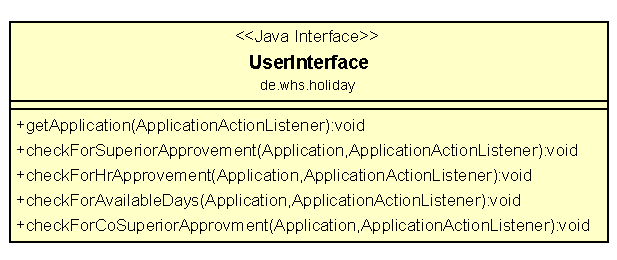
\includegraphics[width=0.7\linewidth]{Bilder/SchnittstelleUserInterface}
\caption{Die Schnittstelle UserInterface}
\label{fig:SchnittstelleUserInterface}
\end{figure}

Abbildung \ref{fig:SchnittstelleUserInterface} zeigt das UserInterface worüber die Interaktion mit dem Endanwender realisiert wird. Die Funktionen repräsentieren dabei die verschiedenen Prozessschritte wie beispielsweise "`Genehmigung durch Vorgesetzten"' oder "`Prüfung ausreichend freier Urlaubstage"'. In unserer Anwendung gibt es zwei Implementierungen für das Interface: Eine Konsolenanwendung und eine GUI die wir in Swing realisiert haben.

\begin{figure}[H]
\centering
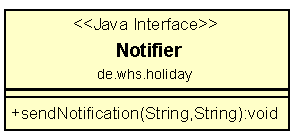
\includegraphics[width=0.35\linewidth]{Bilder/SchnittstelleNotifier}
\caption{Die Schnittstelle Notifier}
\label{fig:SchnittstelleNotifier}
\end{figure}

Zum Verschicken von Benachrichtigungen haben wir die Schnittstelle Notifier (s. Abbildung \ref{fig:SchnittstelleNotifier}) definiert. Für eine reale Unternehmensanwendung könnte man sich hier beispielsweise einen E-Mail-Dienst vorstellen. In unserer Anwendung haben wir die Benachrichtigung über eine Ausgabe in der GUI realisiert.

\begin{figure}[H]
\centering
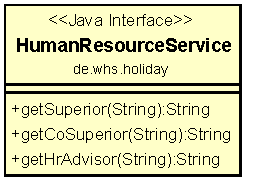
\includegraphics[width=0.3\linewidth]{Bilder/SchnittstelleHumanResourceService}
\caption{Die Schnittstelle HumanResourceService}
\label{fig:SchnittstelleHumanResourceService}
\end{figure}

Abbildung \ref{fig:SchnittstelleHumanResourceService} zeigt die Schnittstelle HumanResourceService, die es uns ermöglicht den Vorgesetzten, Stellvertreter und zuständigen Personalsachbearbeiter für den Antragssteller zu ermitteln. In der Realität könnte man hier beispielsweise das Active-Directory des Unternehmens einbinden. Für unseren Prototyp haben wir die Personalhierarchie unseres Beispielunternehmens statisch hinterlegt.

\subsection{Business Workflow}

\subsubsection{Benutzerdefinierte Aufgabe: Notification}
Um die Benachrichtigung des Mitarbeiters als einzelnen Prozessschritt in unserem BPMN-Diagramm zu realisieren fehlte uns im Standard ein entsprechender Aufgabentyp. Daher haben wir diesen als benutzerdefinierte Aufgabe erstellt. Diese muss ein einer Konfigurationsdatei definiert werden, auf die dann innerhalb der drools.rulebase.conf wie folgt verwiesen werden kann:
\begin{lstlisting}
drools.workDefinitions = HolidayWorkDefinitions.wid WorkDefinitions.conf
\end{lstlisting}

Die Definition für unsere benutzerdefinierte Aufgabe haben wir in der HolidayWorkDefinitions.wid wie folgt vorgenommen:

\begin{lstlisting}
import org.drools.core.process.core.datatype.impl.type.StringDataType;
[
  // the Notification work item
  [
    "name" : "Notification",
    "parameters" : [
      "Message" : new StringDataType(),
      "From" : new StringDataType(),
      "To" : new StringDataType()
    ],
    "displayName" : "Notification",
    "icon" : ""
  ]
]
\end{lstlisting}

Anschließend steht diese Aufgabe im Prozessdesigner als "`Custom Task"' zur Verfügung und kann innerhalb der Prozessdefinition wie die üblichen Elemente verwendet werden:

\begin{figure}[H]
\centering
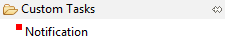
\includegraphics[width=0.4\linewidth]{Bilder/NotificationCustomTask}
\caption{Der CustomTask Notification}
\label{fig:NotificationCustomTask}
\end{figure}


\subsubsection{Der Workflow}
Der Workflow startet mit einem Urlaubsantrag (application), der die initialen Daten für den Prozess mitbringt. Der erste Knoten \textit{holiday type} ist ein Exklusives Oder und unterscheidet anhand des Urlaubstyps und der gewünschten Anzahl Urlaubstage, ob dieser automatisch abgelehnt (rechts, default), automatisch (links) oder manuell (mittig) genehmigt werden muss. Die beiden automatischen Zweige (links und rechts) führen auf direktem Wege durch einen inklusiven Oder-Knoten zum Notification Task und anschließend zum Ende des Workflows.\\
Der mittlere Zweig der manuellen Genehmigung unterscheidet im nächsten Knoten, dem Exklusiven Oder \textit{board member}, ob der Genehmigungsprozess durch Vorgesetzte und den Leiter der Personalabteilung übersprungen werden darf (links). Dies ist der Fall, wenn die beantragende Person Vorstandsmitglied ist und weniger als 5 Tage Urlaub beantragt. Sollte dies nicht der Fall sein ist der nächste Knoten ein Inklusives Oder. In jedem Fall wird von dort aus der Zweig zur Genehmigung durch den Vorgesetzten (mitte) durchlaufen. Sollten mehr als 20 Tage Urlaub beantragt werden, so wird ebenfalls der Zweig zur Genehmigung durch den Leiter der Personalabteilung durchlaufen (rechts). Diese beiden Zweige können parallel abgearbeitet werden, weshalb das Inklusive Oder \textit{additional HR} notwendig ist. Die Genehmigungen werden jeweils durch User Tasks abgebildet.

Im rechten Zweig ist dieser dem Leiter der Personalabteilung zugewiesen. Wichtig ist, dass im Anschluss dieser Zweig mit dem mittleren synchronisiert wird.

\begin{figure}[H]
\centering
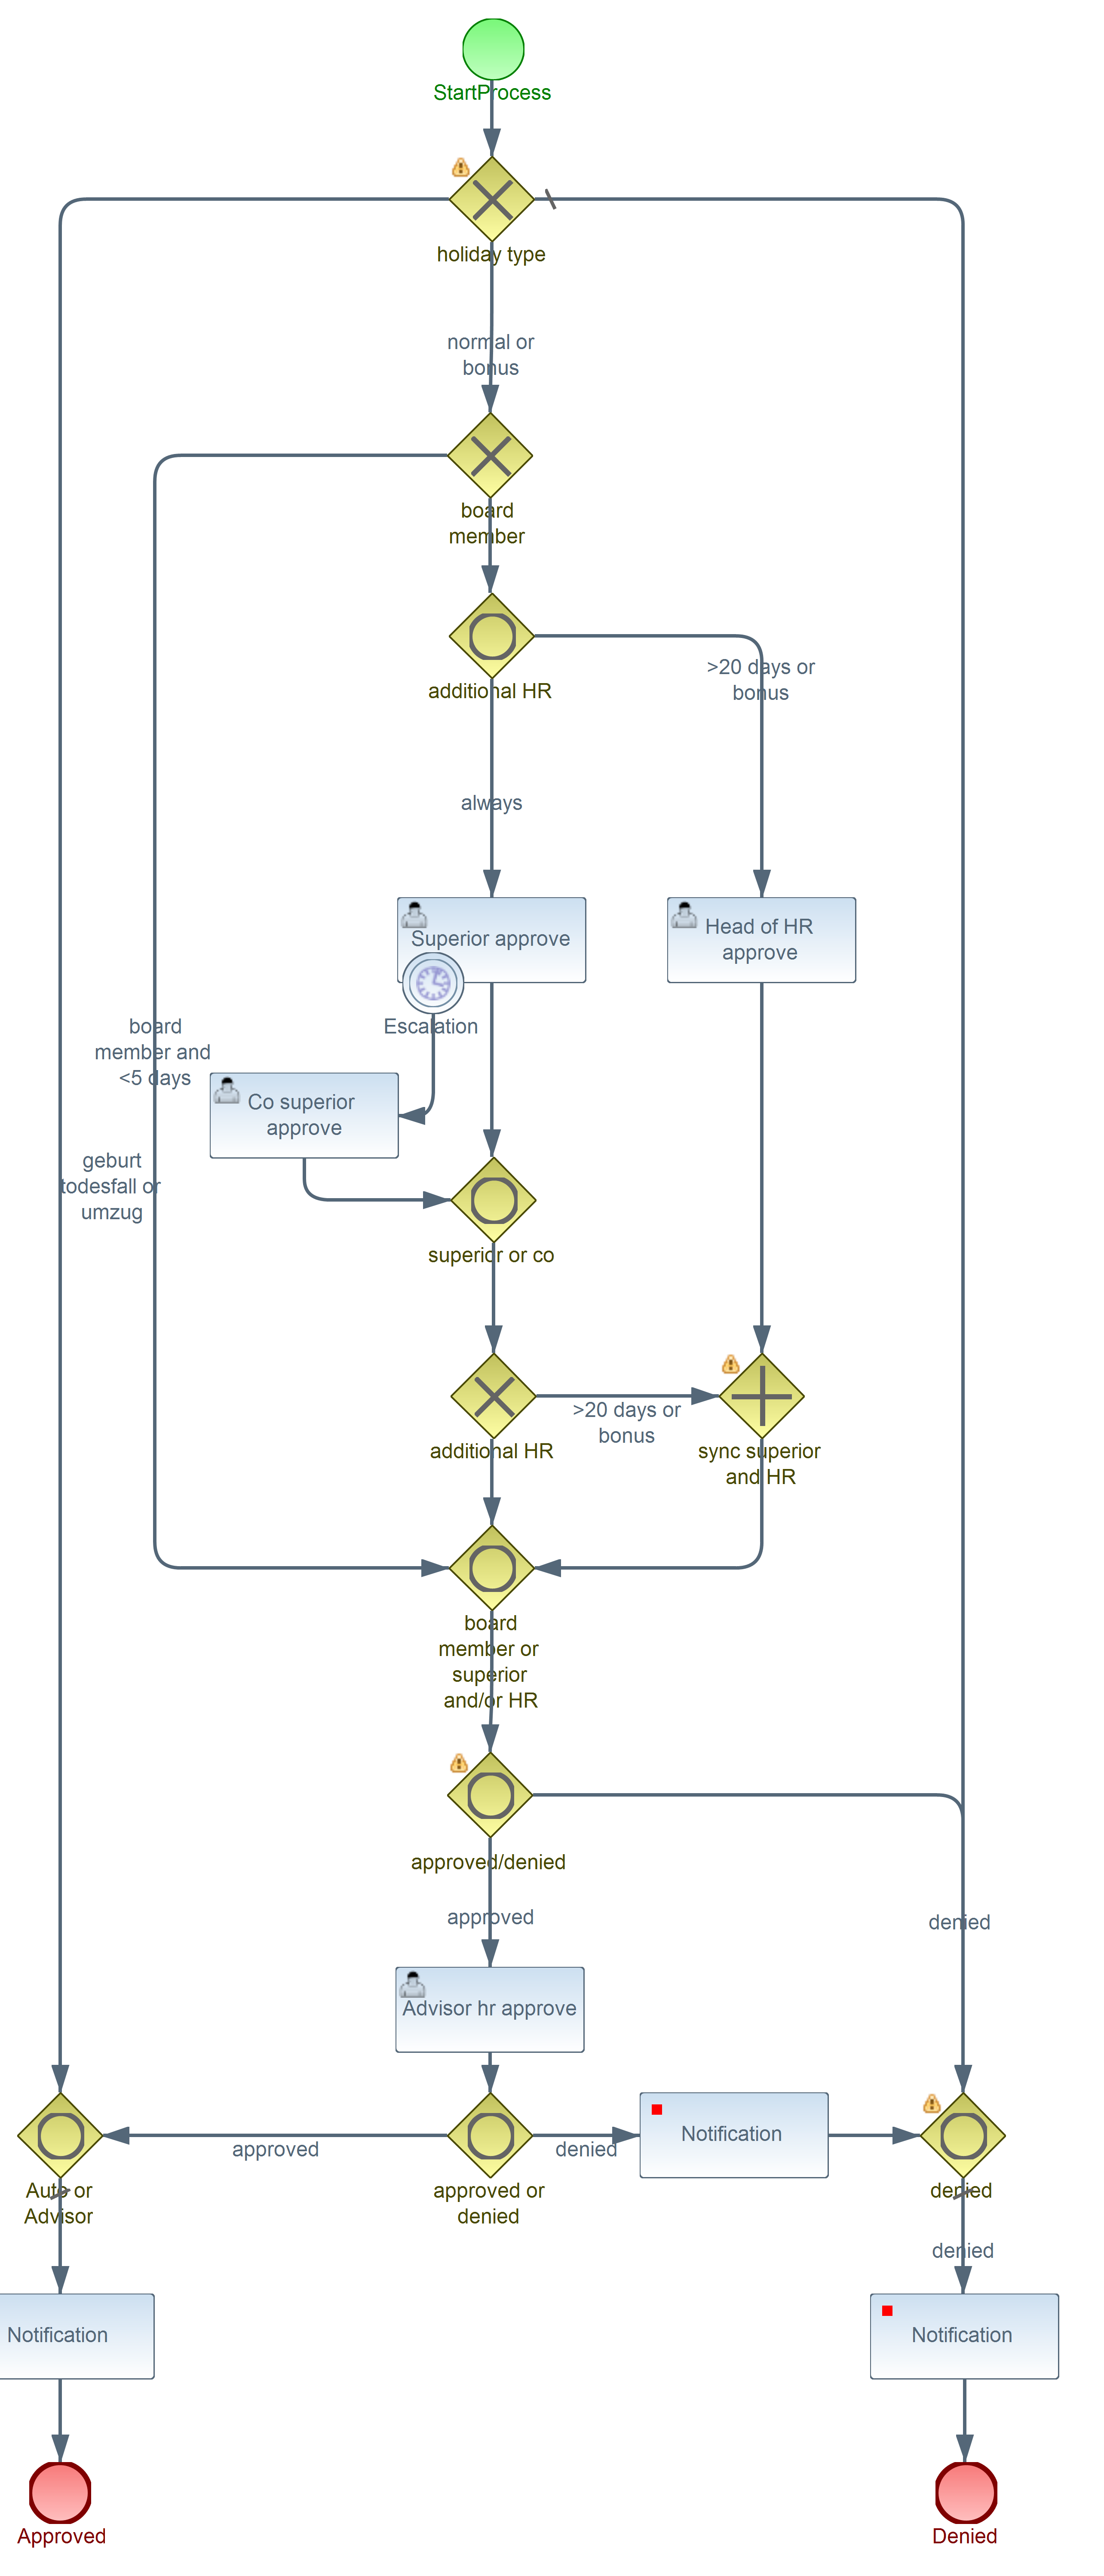
\includegraphics[width=0.75\linewidth]{Bilder/Urlaubsantrag}
\caption{Unser Workflow zur Urlaubsgenehmigung}
\label{fig:Urlaubsantrag}
\end{figure}


\subsection{Benutzeroberfläche}
In diesem Abschnitt wollen wir unsere Swing-Benutzeroberfläche, die aus insgesamt drei Dialogen besteht, vorstellen.

\subsubsection{StartDialog}
Über den StartDialog kann der Mitarbeiter einen neuen Urlaubsgenehmigungsprozess starten. Dazu muss er seinen Namen, die Anzahl der Urlaubstage und den Typ seines Urlaubs eingeben. Über die Combobox kann er zwischen den vier Möglichkeiten Normal, Umzug, Geburt- oder Todesfall und Bonus auswählen.

\begin{figure}[H]
	\centering
	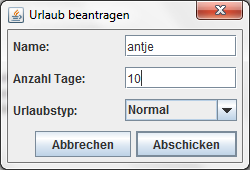
\includegraphics[width=0.4\linewidth]{Bilder/DialogUrlaubBeantragen}
	\caption{Screenshot des StartDialoges}
	\label{fig:DialogUrlaubBeantragen}
\end{figure}

Durch einen Klick auf den Button Abschicken wird ein neuer Prozess gestartet. Alternativ kann der Mitarbeiter den Vorgang auch abbrechen.

\subsubsection{ApproveDialog}
Der ApproveDialog wird verwendet um einen Urlaubsantrag entweder zu genehmigen oder abzulehnen. Da diese Entscheidung in unserem Prozess an mehreren Stellen nötig ist, kommt der Dialog auch entsprechend mehrmals zum Einsatz.

Zunächst muss der Urlaubsantrag durch den Vorgesetzten genehmigt werden. Im Fall von Frau Antje ist die entsprechende Vorgesetzte Frau Ennel:

\begin{figure}[H]
	\centering
	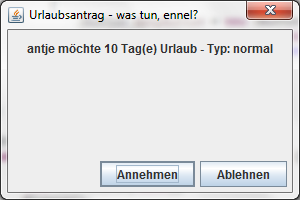
\includegraphics[width=0.5\linewidth]{Bilder/DialogVorgesetzteGenehmigung}
	\caption{Screenshot des ApproveDialogs für die Genehmigung des Vorgesetzten}
	\label{fig:DialogVorgesetzteGenehmigung}
\end{figure}

Sofern der Vorgesetzte den Antrag genehmigt muss dieser in der Personalabteilung durch den zuständigen Sachbearbeiter geprüft werden. Im Fall von Frau Antje ist der zuständige Sachbearbeiter Herr Machfrei:

\begin{figure}[H]
\centering
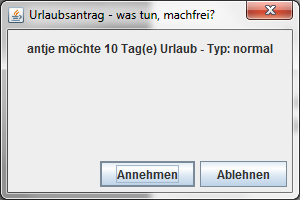
\includegraphics[width=0.5\linewidth]{Bilder/DialogPersonalabteilungGenehmigung}
\caption{Screenshot des ApproveDialos für die Genehmigung in der Personalabteilung}
\label{fig:DialogPersonalabteilungGenehmigung}
\end{figure}

Über die beiden Buttons Annehmen und Ablehnen kann der Antrag genehmigt bzw. abgelehnt werden.

\subsubsection{NotifierDialog}
Über den NotifierDialog wird der Antragssteller benachrichtigt, ob sein Urlaubsantrag genehmigt oder abgelehnt wurde:

\begin{figure}[H]
\centering
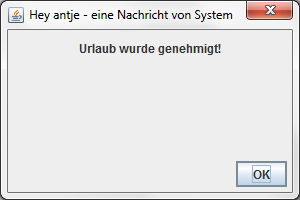
\includegraphics[width=0.5\linewidth]{Bilder/DialogBenachrichtigungGenehmigt}
\caption{Screenshot des NotifierDialogs für einen genehmigten Urlaubsantrag}
\label{fig:DialogBenachrichtigungGenehmigt}
\end{figure}

\begin{figure}[H]
\centering
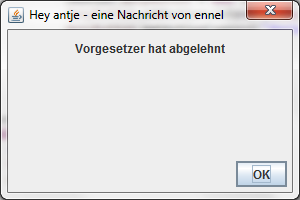
\includegraphics[width=0.5\linewidth]{Bilder/DialogBenachrichtigungAbgelehnt}
\caption{Screenshot des NotifierDialogs für einen abgelehnten Urlaubsantrag}
\label{fig:DialogBenachrichtigungAbgelehnt}
\end{figure}

Über den OK-Button kann die Benachrichtigung geschlossen werden.


